\subsection*{Méthode des différences finies}
\textbf{Principe:}\\
On veut discrétiser une fonction $u(x,y)$ sur un domaine $\Omega$ en utilisant un pas $h$.
\begin{subequations}
    \begin{equation*}
        \underbrace{-\Delta u(x,y)+c(x,y)u(x,y)}_{\mathcal{L}u}=f(x,y)
    \end{equation*}
    \begin{equation*}
        \mathcal{L}u=f\leftrightarrow \mathcal{L}_h\overrightarrow{u_h}=\overrightarrow{f_h}
    \end{equation*}
    \begin{equation*}
        \begin{pmatrix}
             &               & \\
             & \mathcal{L}_h & \\
             &               &
        \end{pmatrix}
        \begin{pmatrix}
            |                    \\
            \overrightarrow{u_h} \\
            |                    \\
        \end{pmatrix}
        =
        \begin{pmatrix}
            |                    \\
            \overrightarrow{f_h} \\
            |                    \\
        \end{pmatrix}
    \end{equation*}
\end{subequations}
\textbf{Discrétisation:}\\
Pour un pas $h=x_{i+1}-x_i=x_i-x_{i-1}$.\\
\underline{Décentré à droite (forward):}
% \begin{subequations}
%     \begin{equation*}
%         \frac{\mathrm{d}u}{\mathrm{d} x}\approx \frac{u(x_i+h)-u(x_i)}{h}\approx \frac{u_{i+1}-u_i}{h}
%     \end{equation*}
%     \begin{equation*}
%         \frac{\partial u}{\partial x}\approx \frac{u_{i+1,j}-u_{i,j}}{h_x}
%     \end{equation*}
%     \begin{equation*}
%         \frac{\partial u}{\partial y}\approx \frac{u_{i,j+1}-u_{i,j}}{h_y}
%     \end{equation*}
% \end{subequations}
\begin{empheq}[box=\fbox]{gather*}
    \frac{\mathrm{d}u}{\mathrm{d} x}\approx \frac{u(x_i+h)-u(x_i)}{h}\approx \frac{u_{i+1}-u_i}{h} \\
    \frac{\partial u}{\partial x}\approx \frac{u_{i+1,j}-u_{i,j}}{h_x}\\
    \frac{\partial u}{\partial y}\approx \frac{u_{i,j+1}-u_{i,j}}{h_y}
\end{empheq}
\underline{Décentré à gauche (backward):}
% \begin{subequations}
%     \begin{equation*}
%         \frac{\mathrm{d}u}{\mathrm{d} x}\approx \frac{u(x_i)-u(x_i-h)}{h}\approx \frac{u_{i}-u_{i-1}}{h}
%     \end{equation*}
%     \begin{equation*}
%         \frac{\partial u}{\partial x}\approx \frac{u_{i,j}-u_{i-1,j}}{h_x}
%     \end{equation*}
%     \begin{equation*}
%         \frac{\partial u}{\partial y}\approx \frac{u_{i,j}-u_{i,j-1}}{h_y}
%     \end{equation*}
% \end{subequations}
\begin{empheq}[box=\fbox]{gather*}
    \frac{\mathrm{d}u}{\mathrm{d} x}\approx \frac{u(x_i)-u(x_i-h)}{h}\approx \frac{u_{i}-u_{i-1}}{h} \\
    \frac{\partial u}{\partial x}\approx \frac{u_{i,j}-u_{i-1,j}}{h_x}\\
    \frac{\partial u}{\partial y}\approx \frac{u_{i,j}-u_{i,j-1}}{h_y}
\end{empheq}
\underline{Centré (différences finies):}
% \begin{subequations}
%     \begin{equation*}
%         \frac{\mathrm{d}u}{\mathrm{d} x}\approx \frac{u(x_i+h)-u(x_i-h)}{2h}\approx \frac{u_{i+1}-u_{i-1}}{2h}
%     \end{equation*}
%     \begin{equation*}
%         \frac{\partial u}{\partial x}\approx \frac{u_{i+1,j}-u_{i-1,j}}{2h_x}
%     \end{equation*}
%     \begin{equation*}
%         \frac{\partial u}{\partial y}\approx \frac{u_{i,j+1}-u_{i,j-1}}{2h_y}
%     \end{equation*}
% \end{subequations}
\begin{empheq}[box=\fbox]{gather*}
    \frac{\mathrm{d}u}{\mathrm{d} x}\approx \frac{u(x_i+h)-u(x_i-h)}{2h}\approx \frac{u_{i+1}-u_{i-1}}{2h} \\
    \frac{\partial u}{\partial x}\approx \frac{u_{i+1,j}-u_{i-1,j}}{2h_x}\\
    \frac{\partial u}{\partial y}\approx \frac{u_{i,j+1}-u_{i,j-1}}{2h_y}
\end{empheq}
\underline{Deuxième ordre:}
% \begin{subequations}
%     \begin{equation*}
%         \frac{\mathrm{d}^2u}{\mathrm{d} x^2}\approx \frac{u(x_i-h)-2u(x_i)+u(x_i+h)}{h^2}\approx \frac{u_{i-1}-2u_i+u_{i+1}}{h^2}
%     \end{equation*}
%     \begin{equation*}
%         \frac{\partial^2 u}{\partial x^2}\approx \frac{u_{i-1,j}-2u_{i,j}+u_{i+1,j}}{h_x^2}
%     \end{equation*}
%     \begin{equation*}
%         \frac{\partial^2 u}{\partial y^2}\approx \frac{u_{i,j-1}-2u_{i,j}+u_{i,j+1}}{h_y^2}
%     \end{equation*}
%     \begin{equation*}
%         \frac{\partial^2 u}{\partial x \partial y}\approx \frac{u_{i+1,j+1}-u_{i+1,j-1}-u_{i-1,j+1}+u_{i-1,j-1}}{4h_xh_y}
%     \end{equation*}
% \end{subequations}
\begin{empheq}[box=\fbox]{gather*}
    \frac{\mathrm{d}^2u}{\mathrm{d} x^2}\approx \frac{u(x_i-h)-2u(x_i)+u(x_i+h)}{h^2}\approx \frac{u_{i-1}-2u_i+u_{i+1}}{h^2} \\
    \frac{\partial^2 u}{\partial x^2}\approx \frac{u_{i-1,j}-2u_{i,j}+u_{i+1,j}}{h_x^2}\\
    \frac{\partial^2 u}{\partial y^2}\approx \frac{u_{i,j-1}-2u_{i,j}+u_{i,j+1}}{h_y^2}\\
    \frac{\partial^2 u}{\partial x \partial y}\approx \frac{u_{i+1,j+1}-u_{i+1,j-1}-u_{i-1,j+1}+u_{i-1,j-1}}{4h_xh_y}
\end{empheq}
\textbf{Exemple 1D:}\\
Soit le problème suivant:
\begin{equation*}
    \left\{
    \begin{aligned}
         & -u''(x)+c(x)u(x)=f(x)\quad \text{dans} \quad \Omega=(0,1) \\
         & u(0)=\alpha                                               \\
         & \lambda u(1)+u'(1)=g\quad (CB:Robin)                      \\
    \end{aligned}
    \right.
\end{equation*}
On sait que $x_1=0$ et donc que \colorbox{orange}{$u_1=\alpha$}. Pour les $x_i$ ont discrétise l'équation
différentielle:
\begin{gather*}
    -\left(\frac{u_{i-1}-2u_i+u_{i+1}}{h^2}\right)+c_iu_i=f_i\\
    -\frac{1}{h^2}u_{i-1}+\frac{1}{h^2}u_i\left(2+h^2c_i\right)-\frac{1}{h^2}u_{i+1}=fi\\
    \colorbox{green}{$\displaystyle\frac{1}{h^2}\left[-u_{i-1}+u_i(2+h^2c_i)-u_{i+1}\right]=f_i$}
\end{gather*}
On sait que $x_N=1$, discrétisée par le technique du point fictif la condition au bord de Robin:
\begin{subequations}
    \begin{equation*}
        \lambda u_N+\frac{u_{N+1}-u_{N-1}}{2h}=g
    \end{equation*}
    \begin{equation*}
        u_{N+1}=2h(g-\lambda u_N)+u_{N-1}
    \end{equation*}
\end{subequations}
En supposant que l'équation différentielle est valide aussi au bord $x_N=1$ on la discrétise:
\begin{equation*}
    -\left(\frac{u_{N-1}-2u_N+u_{N+1}}{h^2}\right)+c_Nu_N=f_N
\end{equation*}
Dans laquelle on substitue $u_{N+1}$:
\begin{gather*}
    -\left(\frac{u_{N-1}-2u_N+2h(g-\lambda u_N)+u_{N-1}}{h^2}\right)+c_Nu_N  =f_N              \\
    -\left(\frac{u_{N-1}-2u_N+2hg-2h\lambda u_N+u_{N-1}}{h^2}\right)+c_Nu_N  =f_N              \\
    -\frac{2}{h^2}u_{N-1}+\frac{1}{h^2}u_N\left(2+2h\lambda+h^2c_N\right)    =f_N+\frac{2g}{h} \\
    \colorbox{yellow}{$\frac{1}{h^2}\left[-2u_{N-1}+u_N(2+2h\lambda+h^2c_N)\right]              =f_N+\frac{2g}{h}$}
\end{gather*}
On obtient donc le système suivant:
\begin{gather*}
    \frac{1}{h^2}
    \resizebox{0.75\columnwidth}{!}{%
        $\left(\begin{tabular}{cccccc}
                \rowcolor{orange}$1$  & $0$        & $0$        & $0$      & $0$            & $0$                  \\
                \rowcolor{green} $-1$ & $2+h^2c_2$ & $-1$       & $0$      & $0$            & $0$                  \\
                \rowcolor{green}$0$   & $-1$       & $2+h^2c_3$ & $-1$     & $0$            & $0$                  \\
                \rowcolor{green}$0$   & $0$        & $0$        & $\ddots$ & $0$            & $0$                  \\
                \rowcolor{green}$0$   & $0$        & $0$        & $0$      & $2+h^2c_{N-1}$ & $-1$                 \\
                \rowcolor{yellow}$0$  & $0$        & $0$        & $0$      & $-2$           & $2+2h\lambda+h^2c_N$ \\
            \end{tabular}\right)$}%
    \cdot
    \left(\begin{smallmatrix}
            u_1    \\
            u_2    \\
            u_3    \\
            \vdots \\
            u_{N-1} \\
            u_N    \\
        \end{smallmatrix}\right)\\
    =
    \resizebox{0.2\columnwidth}{!}{% Add this line
        $\left(\begin{tabular}{c}
                \rowcolor{orange}$\frac{\alpha}{h^2}$ \\
                \rowcolor{green} $f_2$                \\
                \rowcolor{green} $f_3$                \\
                \rowcolor{green} $\vdots$             \\
                \rowcolor{green} $f_{N-1}$            \\
                \rowcolor{yellow} $f_N+\frac{2g}{h}$  \\
            \end{tabular}\right)$}% Add this line
\end{gather*}
\textbf{Exemple 2D:}\\
On veut trouver une approximation numérique de $-\Delta u=f(x,y)$ dans $\Omega=(0,1)\times(0,1)$.
Couvrir $\Omega$ avec un maillage régulier de pas $h_x=h_y=h$:
\begin{figure}[H]
    \centering
    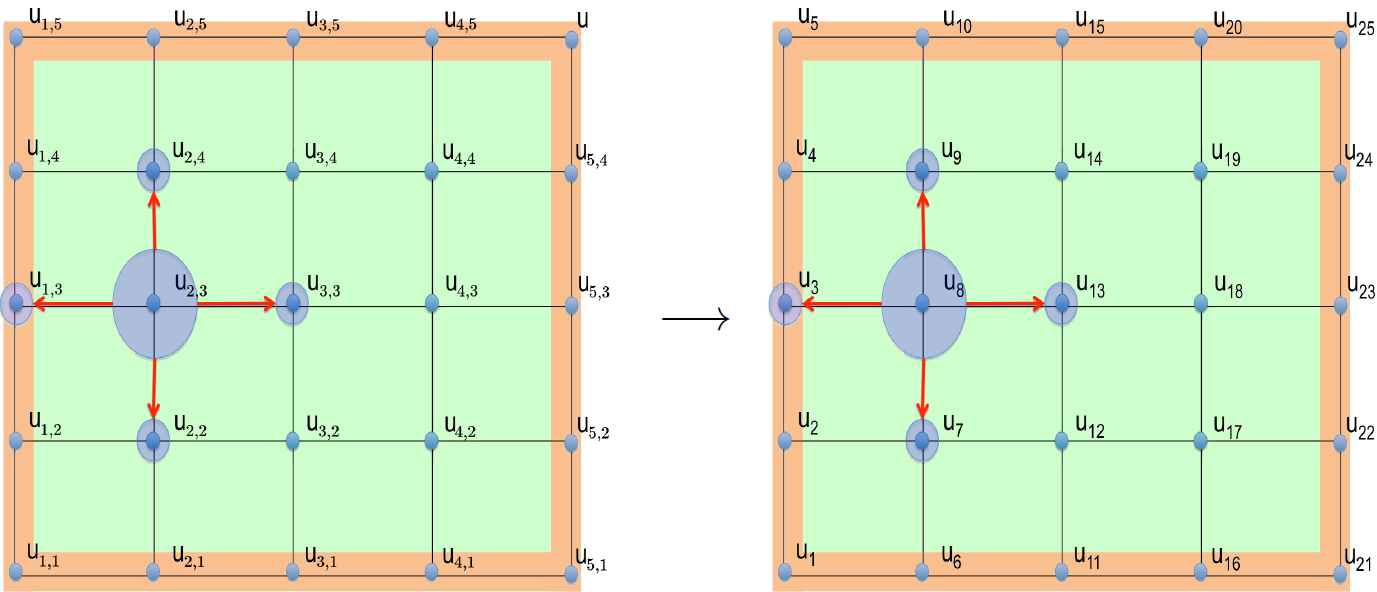
\includegraphics[width=\linewidth]{images/semaine9_diff_finies_2d.png}
\end{figure}
Approchée, l'équation différentielle devient:
\begin{equation*}
    -\Delta u(\overrightarrow{x_{i,j}})\approx\frac{1}{h_x^2}[-u_{i-1,j}+2u_{i,j}-u_{i+1,j}]+\frac{1}{h_y^2}[-u_{i,j-1}+2u_{i,j}-u_{i,j+1}]
\end{equation*}
Comme $h_x=h_y=h$:
\begin{equation*}
    -\Delta u(\overrightarrow{x_{i,j}})\approx\frac{1}{h^2}[4u_{i,j}-u_{i-1,j}-u_{i+1,j}-u_{i,j-1}-u_{i,j+1}]
\end{equation*}
En réecrivant $u_{i,j}\rightarrow u_l$, $l=1,\dots,N$. On a par exemple pour
$\overrightarrow{x}_{2,3}=\overrightarrow{x}_8$:
\begin{equation*}
    -\Delta u(\overrightarrow{x}_8)\approx\frac{1}{h^2}[4u_8-u_3-u_13-u_7-u_9]
\end{equation*}
C'est le stencil à 5 points:
\begin{equation*}
    \frac{1}{h^2}
    \begin{bmatrix}
        \cdot & -1 & \cdot \\
        -1    & 4  & -1    \\
        \cdot & -1 & \cdot \\
    \end{bmatrix}
\end{equation*}



